\documentclass[twocolumn,11pt]{IEEEtran}
\usepackage[verbose,expansion=alltext,stretch=50]{microtype}
\usepackage{graphicx}
\usepackage{booktabs}
\usepackage{hyperref}
\usepackage{xcolor}
\newcommand{\link}[1]{{\color{blue}\href{#1}{#1}}}

\title{DeepSched: A Deep Representation Of Scheduling Policies For Heterogeneous Distributed Systems}

\author{
   \begin{tabular}{c| c| c| c}
       Mohamed Shawky & Remonda Talaat & Mahmoud Adas & Evram Youssef\\
       \texttt{\small{SEC 2, B.N 16}} & \texttt{\small{SEC 1, B.N 20}} & \texttt{\small{SEC 2, B.N 21}} & \texttt{\small{SEC 1, B.N 9}}
   \end{tabular}%
   
   \texttt{\small{\{mohamedshawky911, remondatalaat21, mido3ds, evramyousef\}@gmail.com}}
}%

\markboth{Cairo Uni. CMP Dep. $|$ OS Research $|$ Final Paper $|$ \today}{Shell}

\begin{document}
\maketitle

\begin{abstract}
Task scheduling is one of the core problems in any distributed system. The ability of the system to assign tasks to its different resources to achieve the best possible performance with the least resource consumption is the main challenge in distributed systems research. The heterogeneity of the distributed systems adds another layer of complexity on top of the mentioned problem. The different execution time on different processors and different task dependencies make the scheduling problem very computationally intensive. Usually, researchers and developers turn to greedy-based methods or even recursive optimization methods to reach some optimal or sub-optimal solution. However, due to the nature of the problem, these solutions might take very long time and usually degrade in complex situations. In this work, we propose the idea of scheduling algorithms approximation, where we approximate the complex scheduling algorithms using other models to achieve the same results but with lower execution time. Neural networks are proposed for this task, as they are great function approximators. The complexity of neural networks comes at training time, however they can maintain constant execution time in inference. This constant execution time is relatively low, as it's a simple feedforward process. This makes neural networks a perfect candidate for us, however this comes at a cost of static scheduling scenarios, which is useful in some case such as simulation workflow on supercomputers. The proposed network can achieve almost the same performance of the approximated method (HEFT) on seen data during training and slightly worse performance on unseen data.
\end{abstract}

\section{Introduction}
\IEEEPARstart{T}{he} continuous evolution of computing power and growth of widely-distributed applications and \emph{Internet of Things} (IoT) \cite{inproceedings} have driven our needs for better resource allocation methods. 
The performance of any system critically depends on the algorithms used to schedule tasks on its resources. These systems contain limited resources that should be allocated properly, in order to perform the required tasks with maximum efficiency avoiding starvation and resource exhaustion. 
The general objective of any scheduling technique is to get the best possible performance with a reasonable resource utilization. \\ 

Recently, the heterogeneity of the computational systems has increased tremendously, due to the nature of the applications and the great advances in IoT and distributed systems. A \emph{heterogeneous system} can be defined as a range of resources, different in underlying architecture, targeting different types of computational tasks. The usage of a heterogeneous system has proven to be very efficient in increasing the system performance and reducing the overall power consumption. Recent studies \cite{venkat2014harnessing} show that \emph{heterogeneous system} can outperform the best homogeneous systems by as much as 21\%, with 23\% energy savings and
a reduction of 32\% in Energy Delay Product. These numbers can be improved even more with better task scheduling and resource allocation methods. \\

However, this comes with the problem of complex task scheduling process. The task scheduling problem for a heterogeneous computing system is more complex than that for a homogeneous system, because of the different execution rates of processors and different communication rates among different processors, which add extra layers of complexity to the problem. \\

The first type of methods to turn to is greedy-based methods, where the best possible choice in the current situation is considered. The execution time of these methods rapidly increases with input size and their performance degrades in complex situations. However, the parameters of the scheduling problem in heterogeneous distributed systems make it very suitable for various optimization techniques. Recursive optimization techniques are very efficient in solving many optimization problem. Previous work has investigated the usage of techniques such as \emph{genetic algorithms} \cite{article2} to solve the task scheduling problem. Also, the usage of a progressive decision making techniques such as \emph{Reinforcement Learning} \cite{ORHEAN2018292} for task scheduling in heterogeneous systems has been investigated. \\

In this paper, we investigate the ability of advanced predictive models to learn a representation of static local task scheduling problem. This learned representation is used to approximate the scheduling performance of other scheduling techniques. \emph{Neural Networks} are our best candidate for this task. Neural networks are being used in many fields replacing traditional methods, such as image classification \cite{10.1145/3065386}, object detection \cite{ren2015faster}, neural language modelling \cite{ren2015faster}, image generation \cite{karras2019analyzing} and others. They have proven to be more efficient than other traditional methods. The complexity of the neural networks comes in the development phases, where the network is designed and trained. However, in inference phase, neural networks can achieve very accurate results at high speed. Recent work has been done on optimizing neural network inference through various techniques, such as quantization \cite{choukroun2019lowbit} and pruning \cite{yeom2019pruning}. \\

The recent advances in \emph{Deep Learning} research are considered in designing and training our scheduling network. \emph{Heterogeneous Earliest Time First} (HEFT) \cite{993206} is used as a target, where the network learns to approximate its performance. Also, we include a genetic algorithm experiment for the same problem for comparison. We will discuss our approach to the problem and its limitations.

\section{Related Work}
Since task scheduling in heterogeneous systems is a wide problem, a lot of research has been conducted in this area. Various techniques have been introduced for the problem. These techniques are categorized based on multiple aspects \cite{inbook} and some of which are adapted from task scheduling methods for homogeneous systems.

\subsection{Scheduling Categories}
In this work, we focus on three basic categorizations of heterogeneous task scheduling methods. \\

\subsubsection{Application-Specific vs. System-Specific}
Heterogeneous scheduling methods can be divided into two main categories based on their target metric.

\emph{Application-Specific} scheduling targets task execution speed (performance), where scheduling
decisions are determined based on many parameters including application performance, task inter-dependency and the availability of resources. \emph{System-Specific} scheduling targets resource utilization, where scheduling decisions are based on the percentage of time a resource is available or busy. \\

\subsubsection{Global vs. Local}
Also, heterogeneous scheduling methods can be divided into global and local scheduling.

\emph{Global} scheduling can migrate the tasks from one processor to another, meanwhile \emph{local} scheduling can't migrate, so once a task is assigned to a processor, it stays in its queue.  \\

\subsubsection{Static vs. Dynamic}
Finally, heterogeneous scheduling methods can be divided into static and dynamic scheduling. 

In \emph{static} scheduling, the tasks required to be scheduled are defined before scheduling. However, in \emph{dynamic} scheduling, new tasks can be introduced during the scheduling process.

\subsection{Heterogeneous Earliest Time First (HEFT)}
HEFT \cite{993206} is one of the most well-established algorithms for task scheduling in heterogeneous systems. It's a local static scheduling algorithms, which deals with a \emph{Direct Acyclic Graph} (DAG) of tasks displaying the dependencies between different processes. Each task has a running time for each different machine and a time for communicating the results to children tasks. HEFT is essentially a greedy algorithm, so it's unable make short-term sacrifices for long term benefits. Consequently, HEFT can fail in complex situations. A wide range of algorithms \cite{inbook} follows HEFT further improving the scheduling performance.

\subsection{Optimization Algorithms}
Recent research has been conducted to use optimization algorithms and predictive models to schedule tasks on heterogeneous system, since these algorithms have proven to be very efficient in solving complex computational problems. 
\subsubsection{Genetic Algorithms (GA)}
GA \cite{article2} can be used to efficiently schedule tasks in different systems. It's used for static scheduling, where a fixed population of tasks are scheduled recursively on multiple processors, based on a specific fitness function.
\subsubsection{Reinforcement Learning (RL)}
Also, RL \cite{ORHEAN2018292} has been a strong candidate for the problem, as the scheduling problem can be formulated as an \emph{RL} problem, solved by various \emph{RL} techniques. RL techniques are effective in solving progressive decision making problems, so they are more likely to be used in dynamic scheduling.

\subsection{Neural Networks}
Recent advances in \emph{Deep Learning} have enabled neural networks to dominate many fields, such as computer vision, natural language processing, robotics and others. Neural networks are able to perform perception tasks at a human-level accuracy. Also, neural networks are very efficient in function approximation and representation learning. These properties make neural networks a perfect choice for massive scale automation of many tasks. Some studies even investigated the usage of \emph{Artificial Neural Networks} (ANNs) \cite{article3} in task scheduling in heterogeneous systems. Most of these studies focus on the usage of \emph{Hopfield Nets} \cite{sathasivam2008logic} and \emph{Inhibitor Neurons} \cite{article3}. \\

However, recent advances in \emph{Deep Learning} have come up with new techniques of using neural networks in complex situations. One of the most shiny techniques are \emph{Recurrent Neural Networks} (RNNs) \cite{chung2014empirical}. RNNs have been widely used in many fields such as natural language processing \cite{bahdanau2014neural}, speech recognition \cite{DBLP:journals/corr/AmodeiABCCCCCCD15}, image captioning \cite{DBLP:journals/corr/abs-1810-04020}, time-series prediction \cite{prasad2014deep} and others. They have proven to be very efficient in learning complex temporal information from time-series data. That's why, they are used with sequential data such as videos, speech and text. This makes RNNs our main choice, as we are dealing with sequential data which is the tasks to be scheduled.\\

In this paper, we make use of recent advances in \emph{Deep Learning} such as RNNs and other techniques to learn a deep representation of the scheduling problem and use it to approximate the performance of heterogeneous scheduling methods. 

\section{Methodology}
\subsection{Motivation}
Heterogeneous task scheduling is a relatively new concept, which lacks developers support. It's an active area of research, where many techniques are being developed through time. Being able to achieve the best possible performance on the given tasks, while keeping good utilization of resources is a tedious problem in heterogeneous systems. Aside from being accurate, the scheduling methods have to be fast in its execution, also they should not consume the system resources. 

Heterogeneous scheduling methods are very computationally expensive. However, neural networks are relatively fast in inference and research is being conducted on optimizing inference even more. So, if a neural network can approximate the performance of current scheduling method, it can replace this method in production. 

In this work, we study the ability of neural networks to approximate some heuristic methods and explore its accuracy and execution time against heuristic and approximated methods.

\subsection{Formulation}
First, let us specify the main target of this work. As the task scheduling in heterogeneous distributed system is a vast field with lots of settings and algorithms \cite{inbook}, we choose our scheduling setting to be local and static. The goal of this work is to explore the ability of neural networks to approximate the performance of some well-established scheduling algorithms. In our setting, the algorithms are provided a list of tasks, each has its own execution time on different machines and a set of heterogeneous machines, on which the tasks are executed. We compare the results neural networks to some other heuristic and approximate methods.

Although, we choose local static scheduling, we assume that the neural approximation methods can work in other settings as well.

\subsection{Baseline}
Two baseline methods are considered. We choose \emph{Heterogeneous Earliest Finish Time} (HEFT) \cite{993206} to be our heuristic baseline, as it's one of the widely-used scheduling algorithms in heterogeneous systems. Also, genetic algorithms \cite{article2} is provided as an approximate baseline. \\

\subsubsection{Heterogeneous Earliest Time First (HEFT)}
HEFT \cite{993206} is an old and well-established algorithm for scheduling in heterogeneous systems. It has been used as a baseline in research due to its near-optimal results. Basically, it chooses some process to run on some machine, if the former has the earliest finish time, with considering the special nature of the heterogeneous system. However, HEFT isn't practical for real-world systems, as no-one can know in advance the finish time of a process \\

\subsubsection{Genetic Algorithms}
Genetic algorithms \cite{article2} have proven to be very efficient in solving some of the hardest optimization problem. Previous work on the use of genetic algorithms in task scheduling \cite{article2} is adapted to the heterogeneous setting by adding parameters for execution time of different tasks on different machines.

The targeted \emph{fitness function} will be the average waiting time $W_t$ for all tasks. The fitness function for a specific schedule \emph{S} is given by:
\begin{equation}
\mathcal Fitness(S) = \frac{\sum_{i=1}^{N} W_{ti}}{N}
\end{equation}

\subsection{Neural Networks (Deep Learning)}
The main novel idea of this work is the use of \emph{neural networks} for the scheduling problem. Neural Networks are known to be very good at learning representations and function approximation. In this work, we propose an architecture that can be used to reach a good approximated solution for the scheduling problem. \emph{Offline Optimization} of neural networks is to be used, in order to be able to train the network on scheduling samples and then use the trained network to do inference. We avoid using \emph{online optimization}, as it's slow and we mainly care about execution time of the scheduling method.

Previous work tried to use neural networks to solve scheduling problem through \emph{Hopfield Nets} \cite{sathasivam2008logic} and \emph{Inhibitor Neurons} \cite{article3}. However, we try to make use of the recent advances in \emph{Deep Learning} to redefine the scheduling problem and solve it. 

As mentioned, The provided input is a list of tasks with its information and a set of machines. We want the network to learn an implicit representation of the given tasks and machines. Then, the network learn the mapping between the learned representation and the desired schedule. In other words, the target of the network is to take two input list of information of both tasks and machines and then output for each task, the machine to be executed on, the actual start time and the actual finish time. \\
    
\subsubsection{Architecture}
Our architecture consists of two encoders and one decoder, as shown in Fig.\ref{fig:nn}. \\
The first encoder is a fully convolutional network of \emph{1D} convolutional layers, to which is machines specifications are passed. This encoder learns a representation for the machines to be able to use it later in producing the outputs.

The second encoder is an \emph{Recurrent Neural Network} (RNN) \cite{chung2014empirical}, to which the tasks are passed one by one ordered by the arrival time. This network learns a representation of the tasks preserving the arrival order. RNN is chosen due to its proven effectiveness in dealing with sequential data, as they can learn complex temporal information from time sequences.

The two representations are then stacked and passed to two modules. A classification module which states the machine on which a specific task is executed. A regression module that identifies the actual start time and the actual finish time. Mainly, the two modules consist of \emph{1D} convolutional layers.

\begin{figure}[hp]
    \centering
    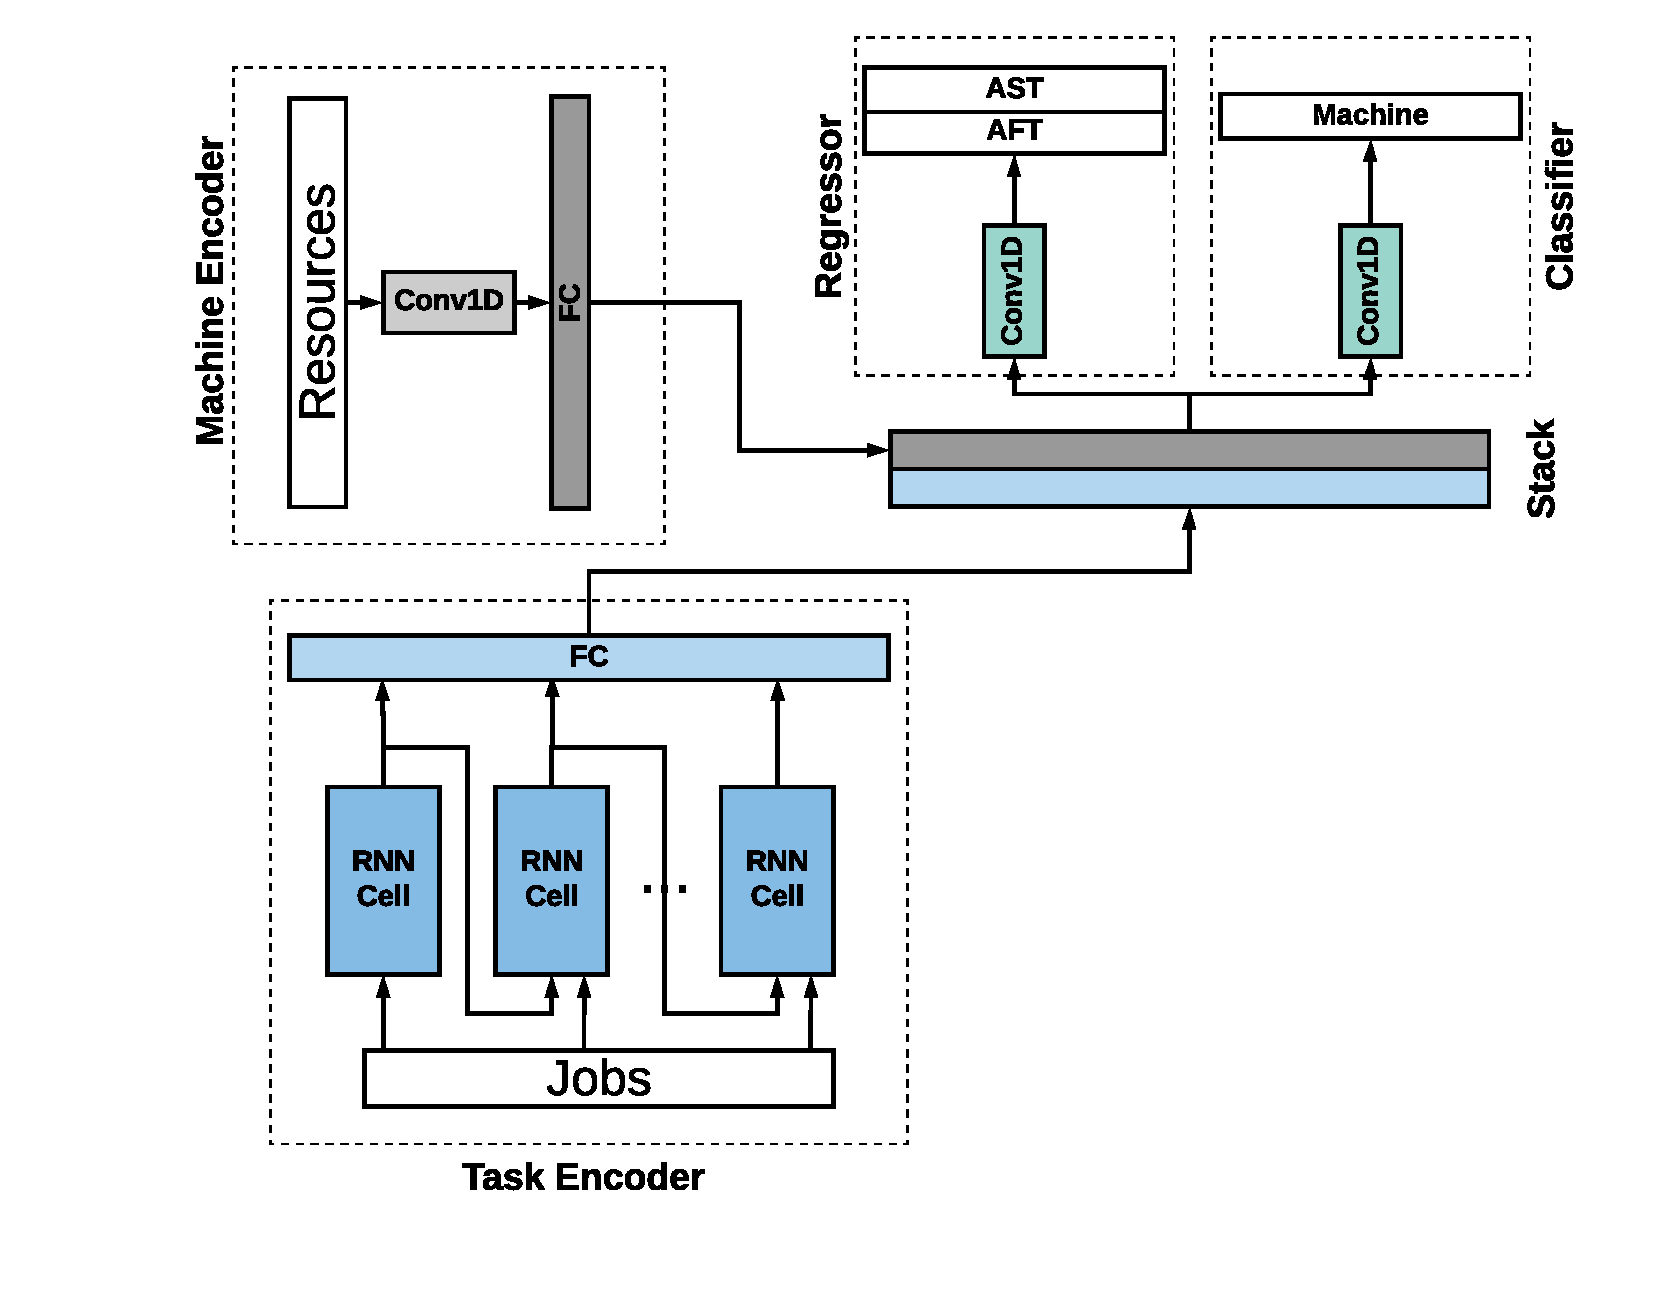
\includegraphics[width=0.45\textwidth]{diagrams/sched_nn}
    \caption{The architecture of the proposed neural network for distributed heterogeneous systems scheduling}
    \label{fig:nn}
\end{figure}
    
\subsubsection{Objective Function}
The cost function defined for this architecture is a sum of two criteria. Categorical cross entropy \emph{(CE)} on the predicted machine to run a specific job $M_p$ and mean square error \emph{(MSE)} on the predicted actual start time $AST_p$ and the predicted actual finish time $AFT_p$. So it can be summarized as follows:
\begin{equation}
\mathcal Loss(L) = CE(M_p, M_t) + MSE(AT_p, AT_t)
\end{equation}
where $M_p$ is the predicted machine, $M_t$ is the ground truth machine, $AT_p$ is the predicted actual time range and $AT_t$ is the ground truth actual time range. \\

\subsubsection{Downsides}
The main downside of the proposed solution is that we have to know the maximum number of machines and the maximum number of tasks to be able to define the network. These numbers are used to define the network and loss function dimensions. 
    
\section{Experimental Setup}
\begin{figure}[hp]
    \centering
    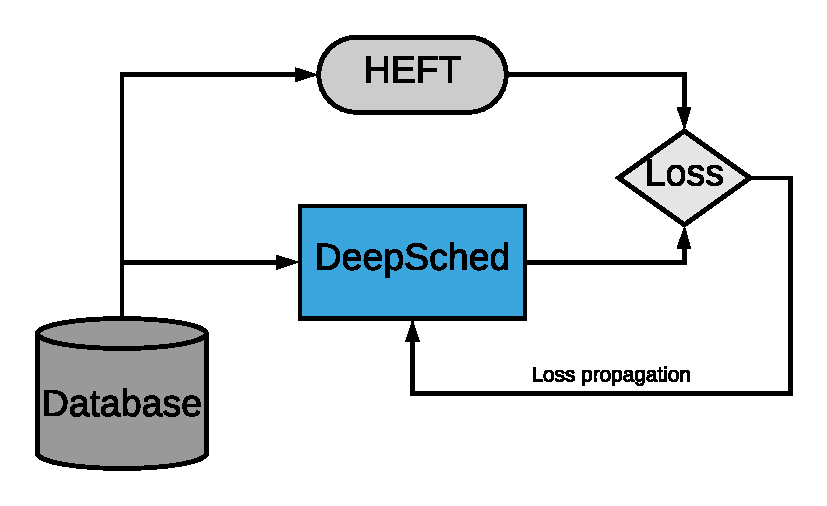
\includegraphics[width=0.45\textwidth]{diagrams/framework}
    \caption{The training framework of DeepSched network. A database of tasks and resources is provided for both network and HEFT. The loss of the network is measured based on HEFT produced schedule.}
    \label{fig:fw}
\end{figure}

Our evaluation methodology of the proposed network is based on comparison with two basic method. One of them is a heuristic method, which is \emph{Heterogeneous Earliest Time First} (HEFT) and the other is an approximate method, which is \emph{Genetic Algorithms} (GA). \\

The results are compared based on the execution time, as well as scheduling performance. For execution time, we measure the total time consumed by scheduling different number of tasks. For scheduling performance, we measure the total turnaround time for all scheduled tasks. Our network is supposed to achieve better execution time with similar performance to HEFT on previously seen data and slightly lower performance on unseen data. 

\subsection{Baseline}
HEFT, which is a heuristic method, is used as a comparison baseline and also to generate the training data, where the network approximates HEFT performance. GA solution, which is an approximate method, is only used as a comparison baseline. \\

\subsubsection{HEFT}
The basic architecture from the original paper \cite{993206} is used in a framework with the proposed neural network shown in Fig.\ref{fig:fw}. HEFT receives some data from a defined database of tasks and resources and produces the output schedule, which is used as labels for the network training data. This way the network can approximate the performance of the HEFT scheduling algorithm by learning to map the input tasks and resources to the schedule produced by HEFT on a large database. \\

\subsubsection{Genetic Algorithms}
The methodology from \cite{article2} is used to develop a genetic algorithm solution for heterogeneous systems. Extra parameters are added to the population to represent the different resources. Also, the execution time is expanded to be a value for each job running on a specific machine, instead of only one execution time value. The used fitness function is the average waiting time \ref{eq:ga}. Random initialization is used along with Crossover. The results of this method are compared to the output of the proposed network.

\subsection{Datasets}
A database of tasks and resources is adapted from \emph{Dataset for Task scheduling in Cloud using CLoudsim} \cite{px5b-b729-20}. The used database consists of $100000$ samples represented as a list of tasks requires to be scheduled. Each sample contains from $486$ to $84654$ tasks, arranged as a \emph{directed acyclic graph} (DAG) to represent the task dependencies and each task has an execution time for each specific processor. Also, the database contains $188$ resource instances (processors), on which the given tasks scheduled. The desired output of such data is to determine, for each task, the optimal processor to run on, the actual start time (AST) and the actual finish time (AFT). 

The provided samples are divided into $90000$ samples for training and validation and $10000$  samples for testing. We maintain diversity in the test data by including different number of tasks in the test samples.

\subsection{Implementation Details}
Our proposed network consists of four main modules.

\subsubsection{Machine Encoder}
This module takes resource details as an input and learns a meaningful representation of them. It consists of one \emph{Conv1D} layer to extract the basic features of each processor, followed by one \emph{fully connected} layer to learn a compact representation of all processors, in order to be passed to the output modules. The common input features for each processor passed to this module are number of processor cores, core frequency and memory capacity. \\

\subsubsection{Task Encoder}
This module takes the time sequence of tasks required to be scheduled and learns a meaningful representation of them through time. \emph{Recurrent neural networks} are used to learn the desired temporal information of the tasks. The module consists of a single \emph{bidirectional gated recurrent unit} (GRU) \cite{chung2014empirical} layer to extract temporal features of each task, followed by one \emph{fully connected} layer to learn a compact representation of all tasks, in order to be passed to the output modules. The common input features for each task passed to this module are arrival time, burst (execution) time for each processor, task priority and memory utilization. \\

The outputs of the previous stages are fused with each other by stacking, in order to form one chunk of information, which is then passed to the two output modules. \\

\subsubsection{Classifier}
The target of this module is to select the optimal running processor for each task amongst the given set of processors. The input to this module is the stacked information of both resources and tasks. It consists of a single \emph{Conv1D} layer, which is used to select running processor for each single task in the form of one hot encoding of the length of resources number. \\

\subsubsection{Regressor}
The target of this module is to predict the actual start time and the actual finish time of each task on the scheduled processor. The input to this module is the stacked information of both resources and tasks. It consists of a single \emph{Conv1D} layer, which is used to regress the actual start and finish times for each task. 

\subsection{Training}
The network is trained on HEFT scheduling outputs. Cross-entropy is used as a classification loss and mean squared error (MSE) is used as a regression loss. The summation of the two losses \ref{eq:l} is used to train the network using gradient descent with \emph{Adam} optimizer and a learning rate of $1e$-$5$. The network is trained for $100$ epochs. The training takes around $1.5$ hours on \emph{Nvidia GTX} $1070$ and around $13$ hours on \emph{Nvidia GTX} $840m$, which is a relatively small time based on both \emph{GPUs} performance.

\subsection{Inference}
Inference is performed on the trained network using both seen and unseen data, in order to compare with both HEFT and genetic algorithms, based on time and performance.

\section{Discussion and Results}
\begin{figure}[hp]
    \centering
    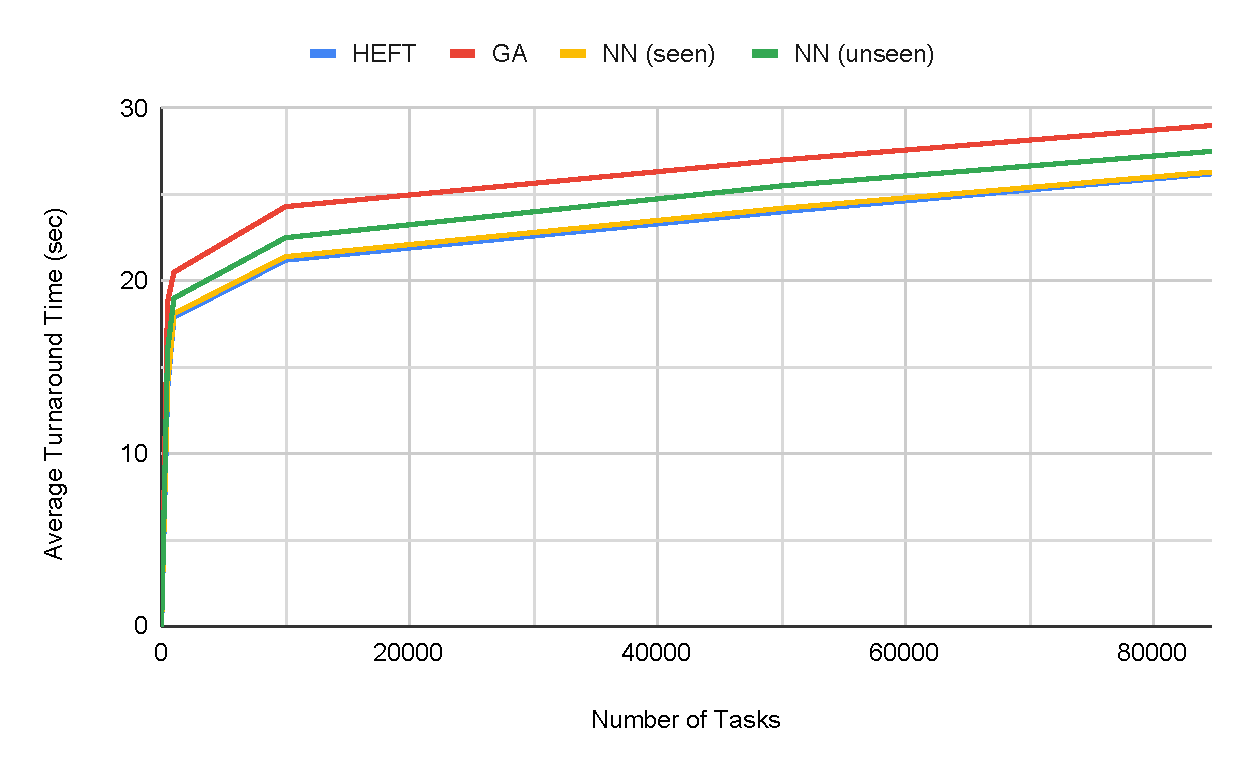
\includegraphics[width=0.45\textwidth]{diagrams/ta_chart}
    \caption{Average turnaround time produced from the three discussed schedulers at different input sizes.}
    \label{fig:ta_chart}
\end{figure}

\subsection{Scheduling Performance}

Fig.\ref{fig:ta_chart} shows the scheduling performance of different scheduling methods at different input sizes. The proposed network shows almost the same average turnaround time as HEFT algorithm for the seen data during training. This is an indicator that the network can learn the underlying representation of the scheduling problem. However, this isn't enough, as the network needs to be tested on unseen data, too. For unseen data, the network shows slightly worse performance than HEFT, but still better than that of genetic algorithms. This indicates the ability of the network to generalize well to other inputs, as long as the network is provided by the same static scenarios and the same maximum number of tasks and resources. \\

These results refer to the network ability to learn a good representation to the input machines and scheduling problem. The network performance degrades with high input sizes, as it's approximating HEFT, which is basically a greedy algorithm and prone to failure at complex situations and large number of input tasks. Genetic algorithms shows similar behaviour too, due to large population size.

\subsection{Execution Time}
\begin{table}
  \caption{Time comparison between the three discussed schedulers at different input sizes. Time is measured in seconds.}
  \label{tab:exec_time}
  \centering
  \begin{tabular}{l l l l}
    \toprule
    Input Size & HEFT & GA & NN \\
    \midrule
    486	& 31.5 & 67.5 & 0.125 \\
    10000 & 305.5 & 602.5 & 0.125 \\
    84654 & 670.0 & 3967.0 & 0.125 \\
    \bottomrule
  \end{tabular}
\end{table}

The main advantage of using neural networks is constant inference time. Once the network is trained, it takes a static execution time in inference, as it's a simple feedforward process that highly supports operation parallelism. Table \ref{tab:exec_time} shows the execution time of the discussed schedulers at 3 different input sizes. These number are produced running on \emph{Intel i5-6600K}. 

We can see that the network consumes constant time in inference with different input sizes. This is because the network is trained on the maximum input length. Also, neural networks operations are highly paralleled, which gives the network a very high speedup when dealing with simple feedforward process, such as network inference. However, HEFT and genetic algorithms execution time increases with input size. GA time increases more rapidly than HEFT, as it's a recursive optimization method but HEFT is a greedy-based method. The performance and static execution time of the network in inference make the network very useful in the situations where static scheduling environment is provided.

\subsection{Results Discussion}
The previous results show that neural networks can approximate a scheduling algorithm for heterogeneous distributed systems, resulting in a significantly good performance and fast execution. The proposed network can perform well, even on unseen data it can produce efficient schedules.

However, this comes with a drawback of static scenarios. The neural network is trained with fixed input size, which is the maximum number of tasks and resources, in our case. At inference time, the input to the network can't exceed that number. So, we have to define the maximum number of tasks to be scheduled, as well as the maximum number of resources. Moreover, the scheduling scenario for the proposed network should be static, where all available tasks should be known before the scheduler starts. 

This gives neural networks a great potential to be a good task scheduler in static scenarios, where the maximum number of tasks and resources are known. The network can be trained offline and then deployed to perform task scheduling. However, in other dynamic scenarios, neural networks might not help much.

\section{Conclusion and Future Work}
In this work, we propose a new approximation method of task scheduling algorithms in heterogeneous distributed system using neural networks. The proposed network is used to approximate HEFT scheduler in static scheduling scenarios. The network can perform as accurate as HEFT on seen data during training and sightly lower performance on unseen data. However, the network can maintain a constant execution time at different input sizes, while HEFT execution time increases rapidly. 

These results show that neural network, which are great function approximators, have the potential to approximate different scheduling methods for heterogeneous distributed systems. They can learn good representation of the scheduling problem, while maintaining constant execution time in inference. 

The main drawback of this method is that static scenarios must be provided. Maximum number to tasks to be scheduled and maximum number of resources must be known before training the network. However, the proposed network is relatively small and doesn't consume much time to train on low or mid-range \emph{GPUs}. \\

In conclusion, It's a trade-off between constant time execution and dynamic systems, where good performance and constant execution time can be achieved in neural networks at static scenarios. This can be useful in some cases such as simulations on supercomputers, where the workflow is static and initially defined. Meanwhile, other solutions, such as RL solutions, can work well in a dynamic environment with no degradation with the complexity of the environment. This is important in IoT-based application, where the system is totally dynamic and can have different events.

\medskip

\bibliographystyle{unsrt}
\bibliography{paper}
    
\end{document}
